% Created 2017-02-12 Sun 22:14
% Intended LaTeX compiler: pdflatex
\documentclass[presentation]{beamer}
\usepackage[utf8]{inputenc}
\usepackage[T1]{fontenc}
\usepackage{graphicx}
\usepackage{grffile}
\usepackage{longtable}
\usepackage{wrapfig}
\usepackage{rotating}
\usepackage[normalem]{ulem}
\usepackage{amsmath}
\usepackage{textcomp}
\usepackage{amssymb}
\usepackage{capt-of}
\usepackage{hyperref}
\usetheme{CambridgeUS}
\usecolortheme{beaver}
\author{Zheng Tian}
\date{}
\title{Lecture 1: What is Econometrics}
\hypersetup{
 pdfauthor={Zheng Tian},
 pdftitle={Lecture 1: What is Econometrics},
 pdfkeywords={},
 pdfsubject={},
 pdfcreator={Emacs 25.1.1 (Org mode 9.0.3)},
 pdflang={English}}
\begin{document}

\maketitle
\begin{frame}{Outline}
\setcounter{tocdepth}{1}
\tableofcontents
\end{frame}


\section*{What is Econometrics}
\label{sec:orgb014773}

\subsection*{Definition of Econometrics}
\label{sec:org10804f8}

Stock and Watson (2015) define Econometrics as

\begin{quote}
At a broad level, econometrics is the science and art of using
economic theory and statistical techniques to analyze economic
data.
\end{quote}


\subsection*{Science or art?}
\label{sec:orgece27f2}

Econometrics is a science because it essentially complies with the
principle of \alert{falsifiability} of scientific research, as Karl Popper
defined.

\begin{frame}[label={sec:org24587a5}]{The reasoning cycle of scientific research}
\begin{figure}[htbp]
\centering
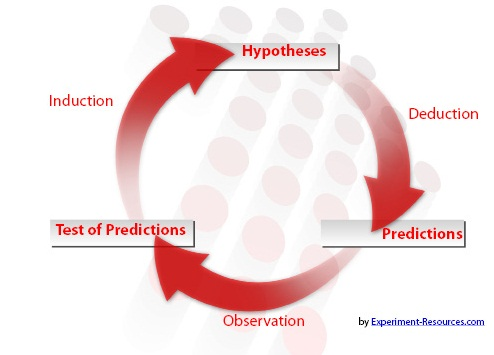
\includegraphics[width=0.5\textwidth]{figure/reasoning-cycle-research.jpg}
\caption{A reasoning cycle of scientific research}
\end{figure}
\end{frame}
\end{document}